\chapter{Appendix} \label{appendix}

\section{Limit Infeasible Curtail Action Experiment Results}

\begin{figure}[H]
	\centering
	\subfloat{}{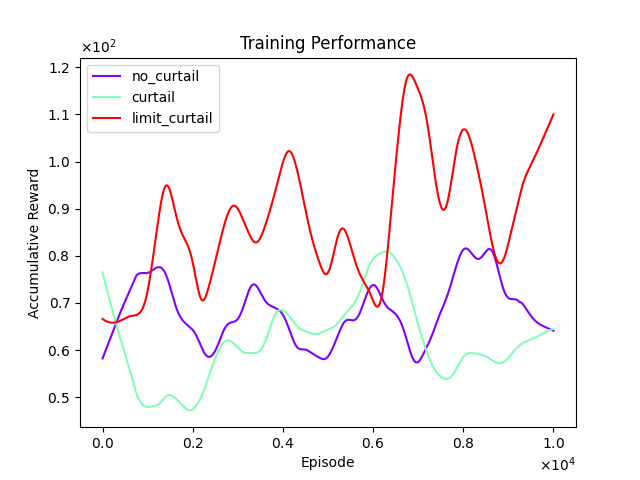
\includegraphics[width=.45\textwidth]{graphs/curtail_limit/training_performance.png}}
	\hskip1ex
	\subfloat{}{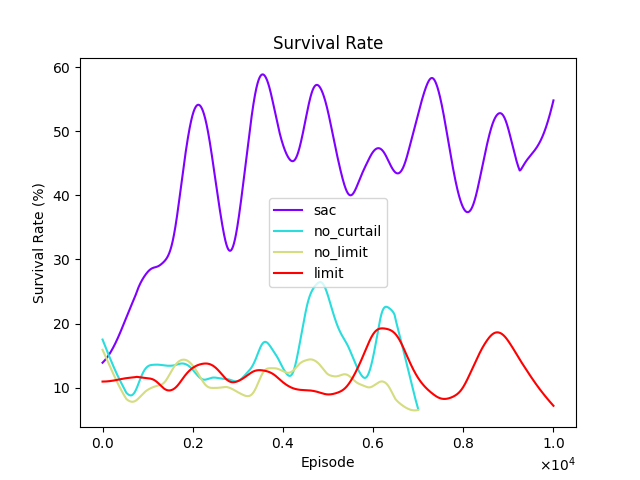
\includegraphics[width=.45\textwidth]{graphs/curtail_limit/survival_rate.png}} 
	\vfill
	\subfloat{}{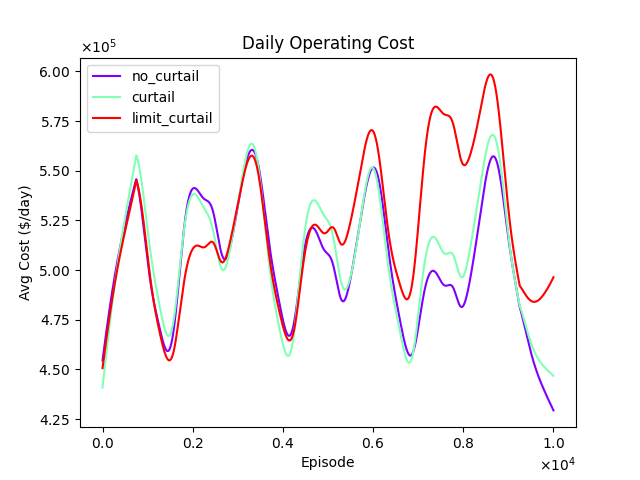
\includegraphics[width=.45\textwidth]{graphs/curtail_limit/daily_cost.png}} \hskip1ex
	\subfloat{}{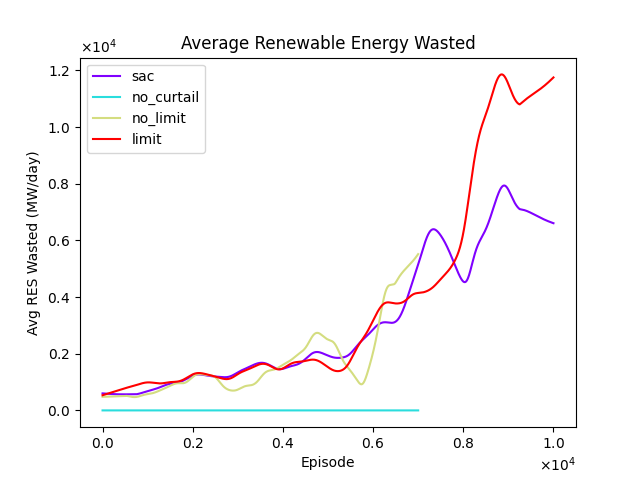
\includegraphics[width=.45\textwidth]{graphs/curtail_limit/res_wasted.png}} 
	\caption{Training Results of the Experiments concerning Limit Infeasible Curtail Actions.}
	\label{fig:curtail-train}
\end{figure}

\begin{table}[ht]
	\centering
	\begin{tabularx}{\textwidth}{|l|X|X|X|X|X|}
		\hline
		\textbf{Model} & \textbf{Avg. Accumulative Reward}& \textbf{Avg. Length (Steps)} & \textbf{Avg Daily Operating Cost (€)} & \textbf{Avg. Renewables Wasted (MW/day)} & \textbf{Total Time (Seconds)}\\
		\hline
		no\_curtail & 68.87 & 225.46 & 533238.32 & 0.0 & 812.81\\
		curtail & 60.81 & 108.27 & 551028.29 & 4565.01 & 510.97 \\
		limit\_curtail & 78.62 & 759.82 & 575798.57 & 7640.76 & 2329.76 \\
		\hline
	\end{tabularx}
	\caption{Validation Results of the Experiments concerning Limit Infeasible Curtail Actions.}
	\label{fig:curtail-val}
\end{table}

\section{Curtailment Lower Limit Smoothing}

\begin{figure}[H]
	\centering
	\subfloat{}{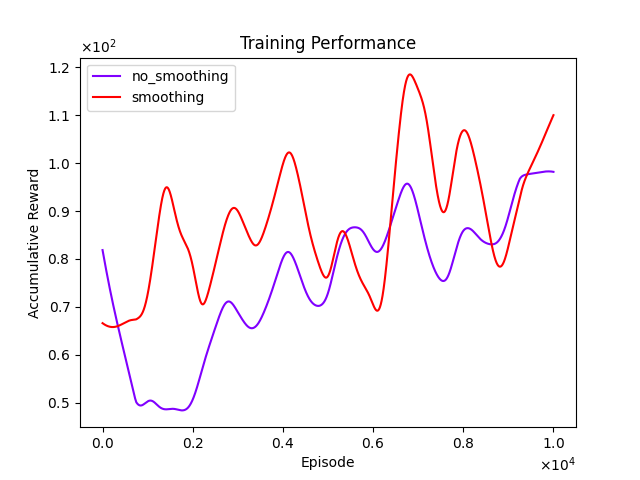
\includegraphics[width=.45\textwidth]{graphs/curtail_smooth/training_performance.png}}
	\hskip1ex
	\subfloat{}{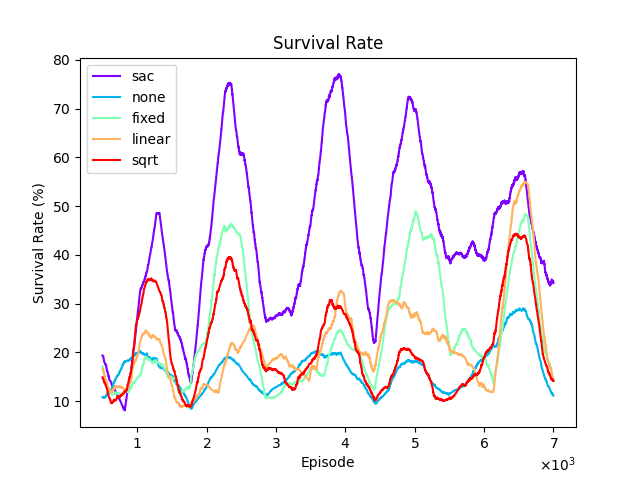
\includegraphics[width=.45\textwidth]{graphs/curtail_smooth/survival_rate.png}} 
	\vfill
	\subfloat{}{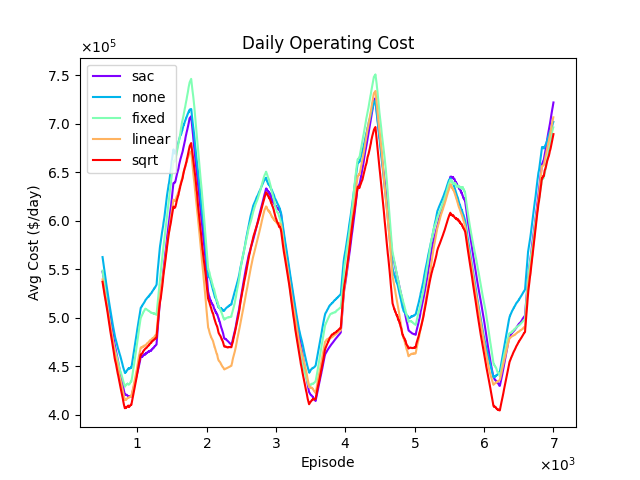
\includegraphics[width=.45\textwidth]{graphs/curtail_smooth/daily_cost.png}} \hskip1ex
	\subfloat{}{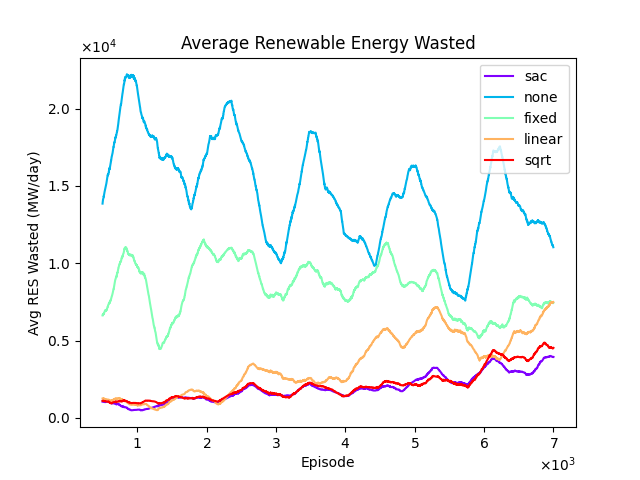
\includegraphics[width=.45\textwidth]{graphs/curtail_smooth/res_wasted.png}} 
	\caption{Training Results of the Experiments concerning Curtailment Lower Limit Smoothing.}
	\label{fig:curtail-smooth-train}
\end{figure}

\begin{table}[ht]
	\centering
	\begin{tabularx}{\textwidth}{|l|X|X|X|X|X|}
		\hline
		\textbf{Model} & \textbf{Avg. Accumulative Reward}& \textbf{Avg. Length (Steps)} & \textbf{Avg Daily Operating Cost (€)} & \textbf{Avg. Renewables Wasted (MW/day)} & \textbf{Total Time (Seconds)}\\
		\hline
		no\_smoothing & 94.91 & 476.48 & 565094.39 & 10106.84 & 3011.93 \\
		smoothing & 78.62 & 759.82 & 575798.57 & 7640.76 & 2329.76 \\
		\hline
	\end{tabularx}
	\caption{Validation Results of the Experiments concerning Limit Infeasible Curtail Actions.}
	\label{fig:curtail-val}
\end{table}

\section{Reward Experiments}

\begin{figure}[H]
	\centering
	\subfloat{}{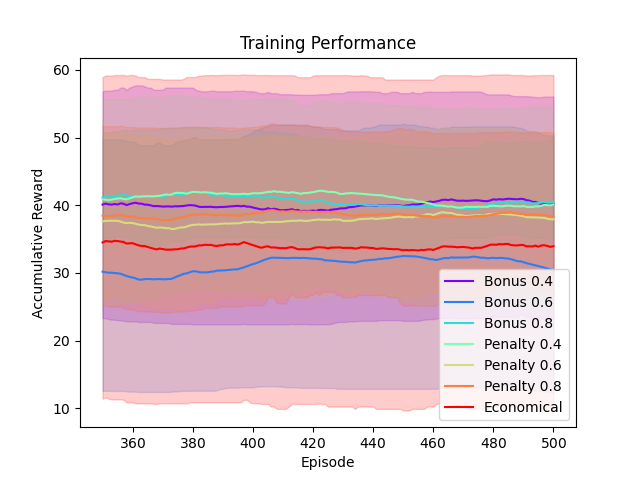
\includegraphics[width=.45\textwidth]{graphs/reward/training_performance.png}}
	\hskip1ex
	\subfloat{}{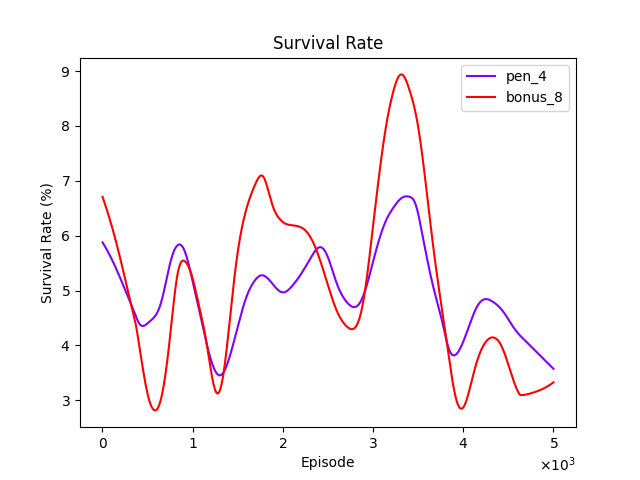
\includegraphics[width=.45\textwidth]{graphs/reward/survival_rate.png}} 
	\vfill
	\subfloat{}{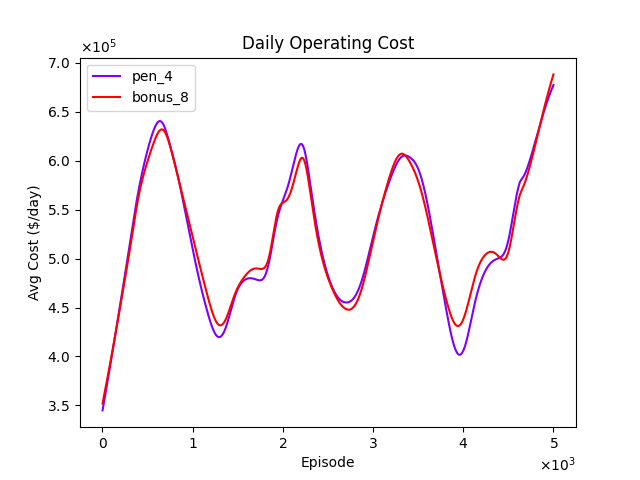
\includegraphics[width=.45\textwidth]{graphs/reward/daily_cost.png}} \hskip1ex
	\subfloat{}{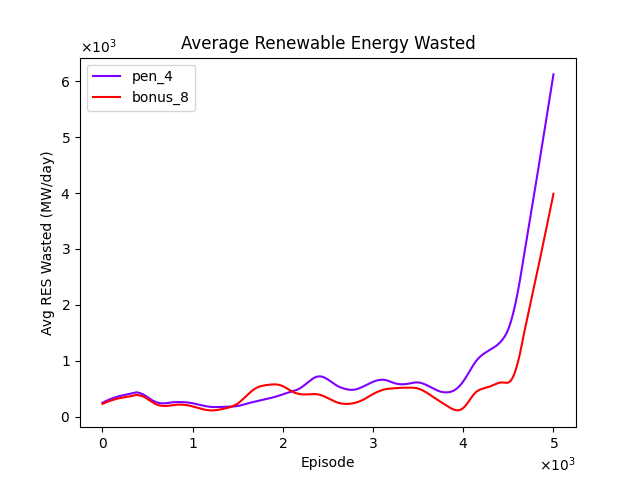
\includegraphics[width=.45\textwidth]{graphs/reward/res_wasted.png}} 
	\caption{Training Results of the best Penalty and Bonus Factor Rewards.}
	\label{fig:reward-best-train}
\end{figure}
\begin{figure}[H]
	\centering
	\subfloat{}{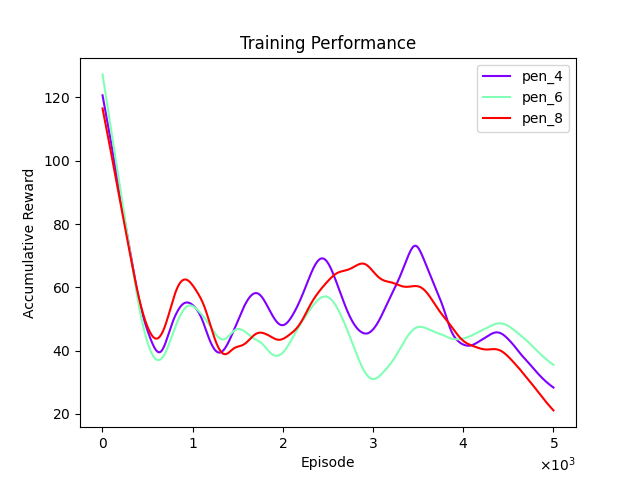
\includegraphics[width=.45\textwidth]{graphs/reward/penalty/training_performance.png}}
	\hskip1ex
	\subfloat{}{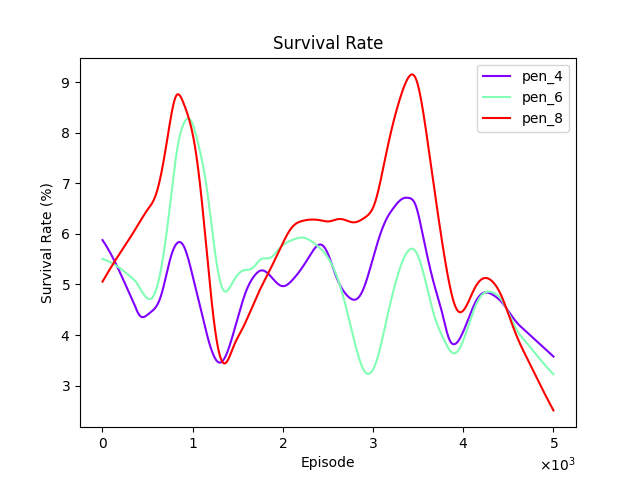
\includegraphics[width=.45\textwidth]{graphs/reward/penalty/survival_rate.png}} 
	\vfill
	\subfloat{}{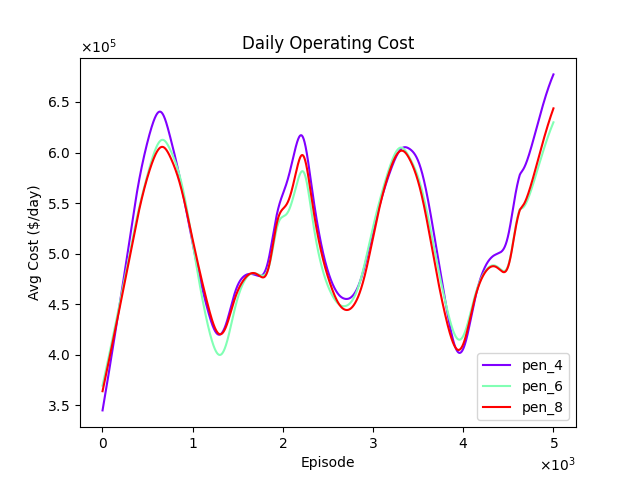
\includegraphics[width=.45\textwidth]{graphs/reward/penalty/daily_cost.png}} \hskip1ex
	\subfloat{}{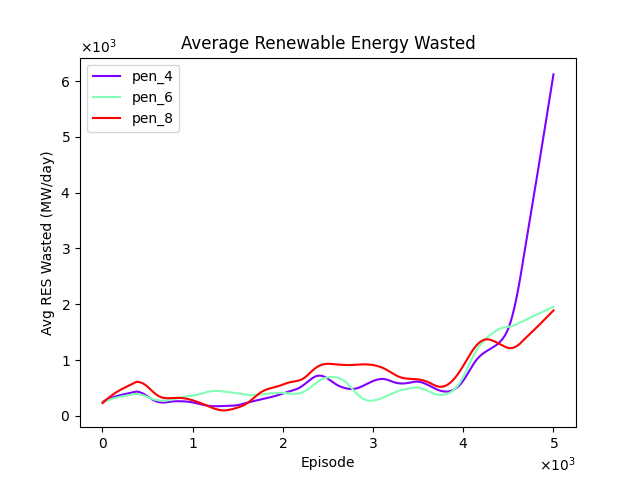
\includegraphics[width=.45\textwidth]{graphs/reward/penalty/res_wasted.png}} 
	\caption{Training Results of the Penalty Factor Rewards.}
	\label{fig:reward-pen-train}
\end{figure}

\begin{figure}[H]
	\centering
	\subfloat{}{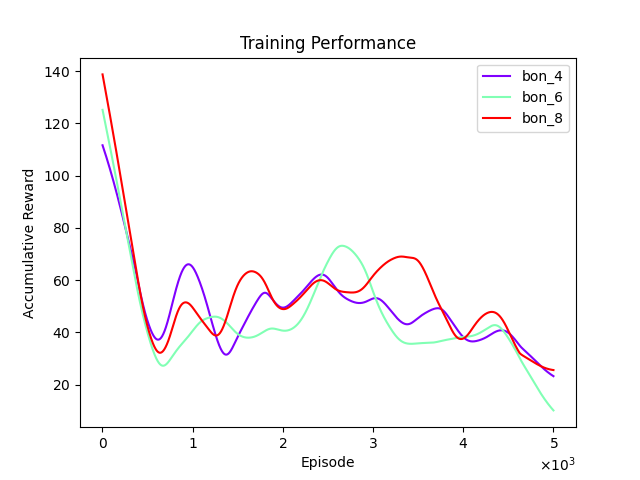
\includegraphics[width=.45\textwidth]{graphs/reward/bonus/training_performance.png}}
	\hskip1ex
	\subfloat{}{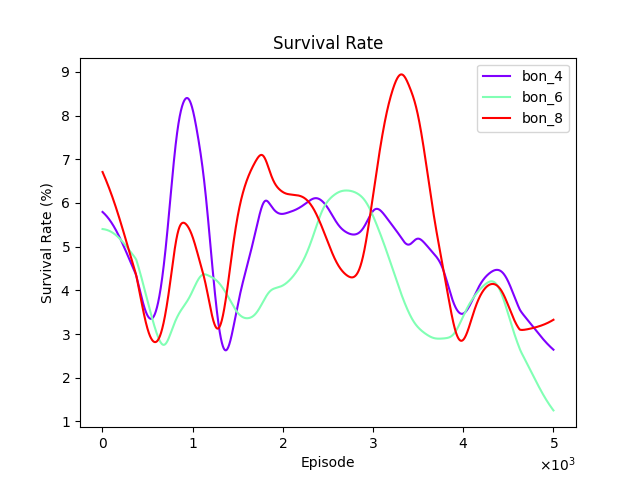
\includegraphics[width=.45\textwidth]{graphs/reward/bonus/survival_rate.png}} 
	\vfill
	\subfloat{}{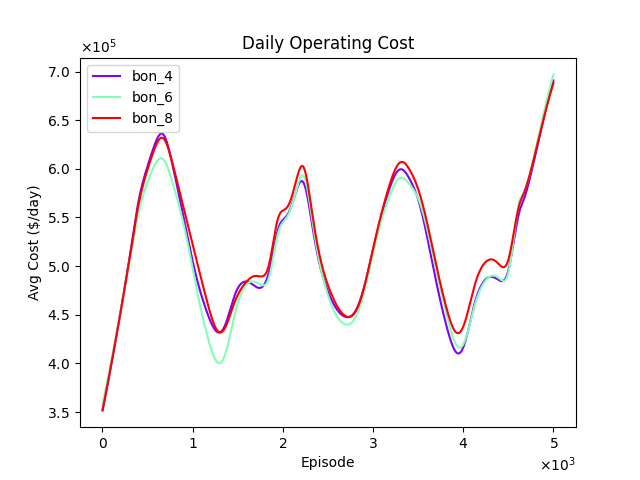
\includegraphics[width=.45\textwidth]{graphs/reward/bonus/daily_cost.png}} \hskip1ex
	\subfloat{}{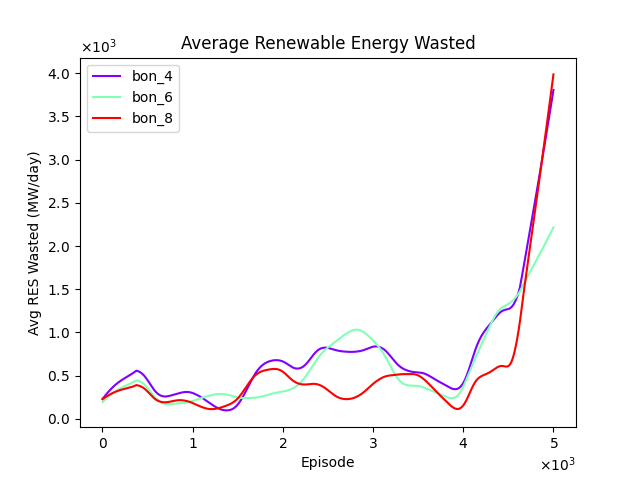
\includegraphics[width=.45\textwidth]{graphs/reward/bonus/res_wasted.png}} 
	\caption{Training Results of the Bonus Factor Rewards.}
	\label{fig:reward-bon-train}
\end{figure}

\begin{table}[ht]
	\centering
	\begin{tabularx}{\textwidth}{|l|X|X|X|X|X|}
		\hline
		\textbf{Model} & \textbf{Avg. Accumulative Reward}& \textbf{Avg. Length (Steps)} & \textbf{Avg Daily Operating Cost (€)} & \textbf{Avg. Renewables Wasted (MW/day)} & \textbf{Total Time (Seconds)}\\
		\hline
		pen\_4 & 40.57 & 80.75 & 565893.63 & 4100.20 & 230.99 \\
		pen\_6 & 37.54 & 81.40 & 558362.82 & 2570.71 & 231.09 \\
		pen\_8 & 38.22 & 76.35 & 555582.14 & 2612.34 & 222.58 \\
		bon\_4 & 40.13 & 76.23 & 565757.16 & 3723.72 & 223.90 \\
		bon\_6 & 30.78 & 55.06 & 566786.07 & 2750.34 & 189.01 \\
		bon\_8 & 40.88 & 96.43 & 560927.60 & 3115.18 & 256.59 \\
		\hline
	\end{tabularx}
	\caption{Validation Results of the Experiments concerning Limit Infeasible Curtail Actions.}
	\label{fig:curtail-val}
\end{table}

\section{Experiments on the \ac{GNN} Parameters \textit{act\_first} and \textit{improved}}

\begin{figure}[H]
	\centering
	\subfloat{}{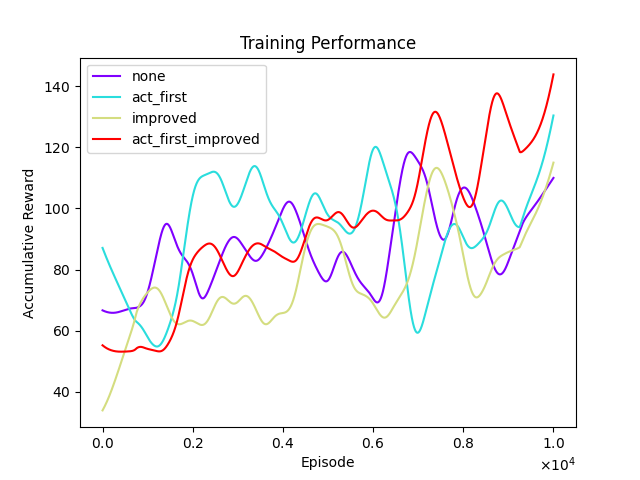
\includegraphics[width=.45\textwidth]{graphs/act_first_improved/training_performance.png}}
	\hskip1ex
	\subfloat{}{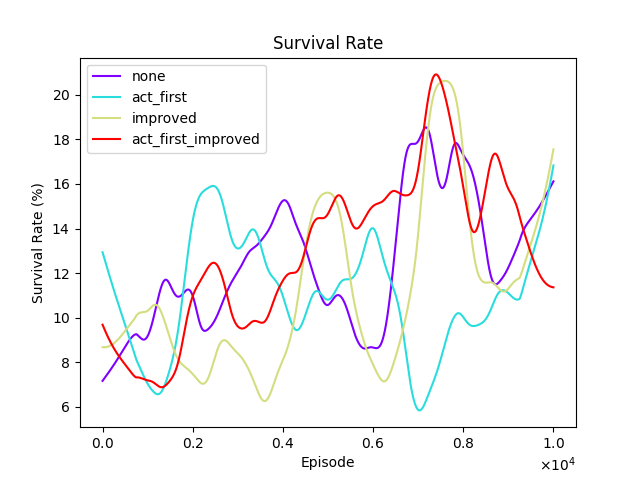
\includegraphics[width=.45\textwidth]{graphs/act_first_improved/survival_rate.png}} 
	\vfill
	\subfloat{}{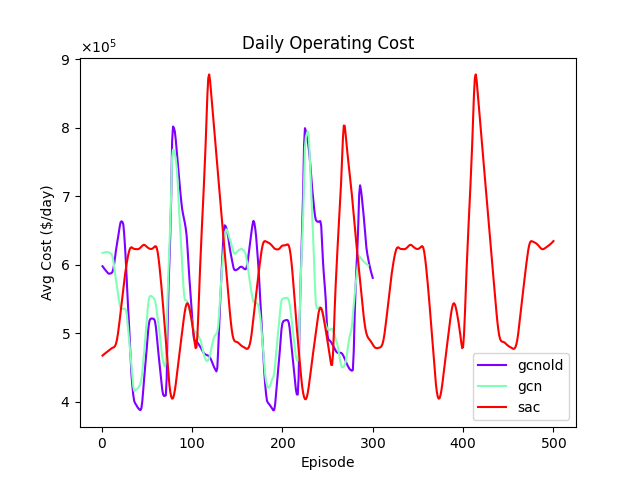
\includegraphics[width=.45\textwidth]{graphs/act_first_improved/daily_cost.png}} \hskip1ex
	\subfloat{}{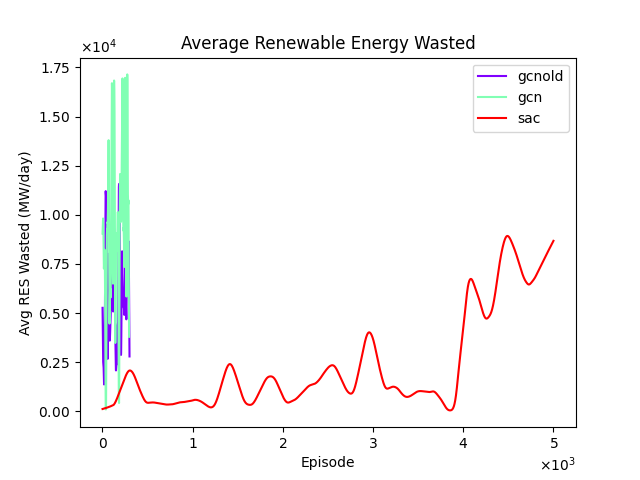
\includegraphics[width=.45\textwidth]{graphs/act_first_improved/res_wasted.png}} 
	\caption{Training Results of the act\_first and improved Parameter Tests.}
	\label{fig:act-first-improved-train}
\end{figure}

\begin{comment}
\begin{table}[ht]
	\centering
	\begin{tabularx}{\textwidth}{|l|X|X|X|X|X|}
		\hline
		\textbf{Model} & \textbf{Avg. Accumulative Reward}& \textbf{Avg. Length (Steps)} & \textbf{Avg Daily Operating Cost (€)} & \textbf{Avg. Renewables Wasted (MW/day)} & \textbf{Total Time (Seconds)}\\
		\hline
		none & & & & & \\
		act\_first & & & & & \\
		improved & & & & & \\
		act\_first\_improved & & & & &  \\
		\hline
	\end{tabularx}
	\caption{Validation Results of the Experiments concerning Limit Infeasible Curtail Actions.}
	\label{fig:curtail-val}
\end{table}
\end{comment}

\section{Experiments on the number of \ac{GNN} layers}

\begin{figure}[H]
	\centering
	\subfloat{}{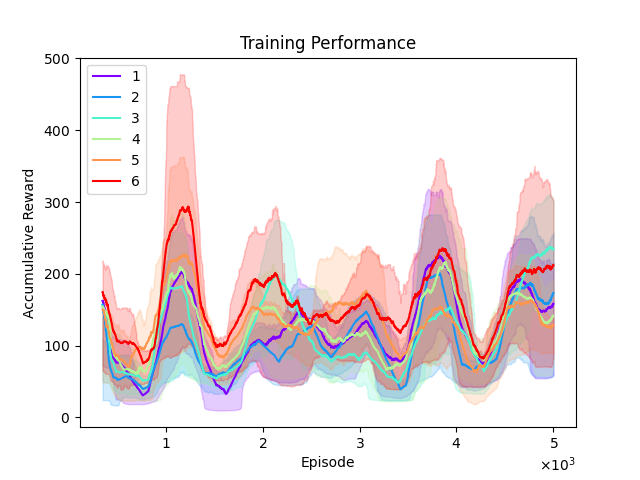
\includegraphics[width=.45\textwidth]{graphs/layers/training_performance.png}}
	\hskip1ex
	\subfloat{}{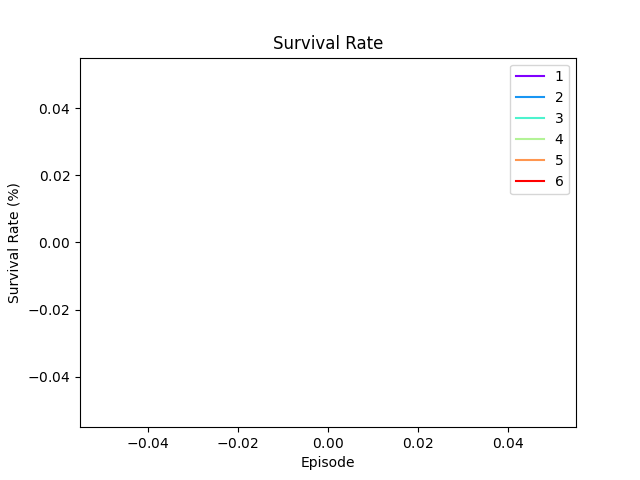
\includegraphics[width=.45\textwidth]{graphs/layers/survival_rate.png}} 
	\vfill
	\subfloat{}{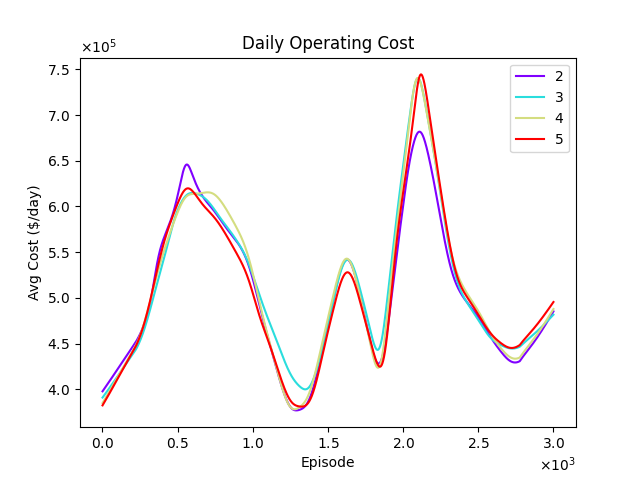
\includegraphics[width=.45\textwidth]{graphs/layers/daily_cost.png}} \hskip1ex
	\subfloat{}{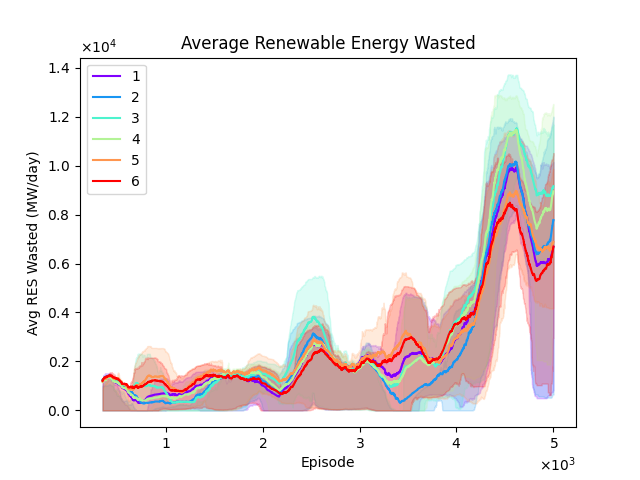
\includegraphics[width=.45\textwidth]{graphs/layers/res_wasted.png}} 
	\caption{Training Results of models with 2, 3, 4 and 5 \ac{GNN} Layers}
	\label{fig:gnn-layers-train}
\end{figure}

\begin{comment}
\begin{table}[ht]
	\centering
	\begin{tabularx}{\textwidth}{|l|X|X|X|X|X|}
		\hline
		\textbf{Model} & \textbf{Avg. Accumulative Reward}& \textbf{Avg. Length (Steps)} & \textbf{Avg Daily Operating Cost (€)} & \textbf{Avg. Renewables Wasted (MW/day)} & \textbf{Total Time (Seconds)}\\
		\hline
		2 & & & & & \\
		3 & & & & & \\
		4 & & & & & \\
		5 & & & & & \\
		\hline
	\end{tabularx}
	\caption{Validation Results of the Experiments concerning Limit Infeasible Curtail Actions.}
	\label{fig:curtail-val}
\end{table}
\end{comment}


\section{Experiments on the number of \ac{GAT} Heads}

\begin{figure}[H]
	\centering
	\subfloat{}{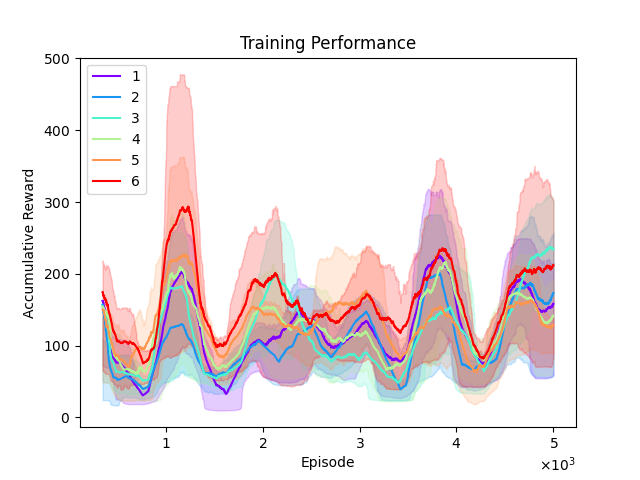
\includegraphics[width=.45\textwidth]{graphs/layers/training_performance.png}}
	\hskip1ex
	\subfloat{}{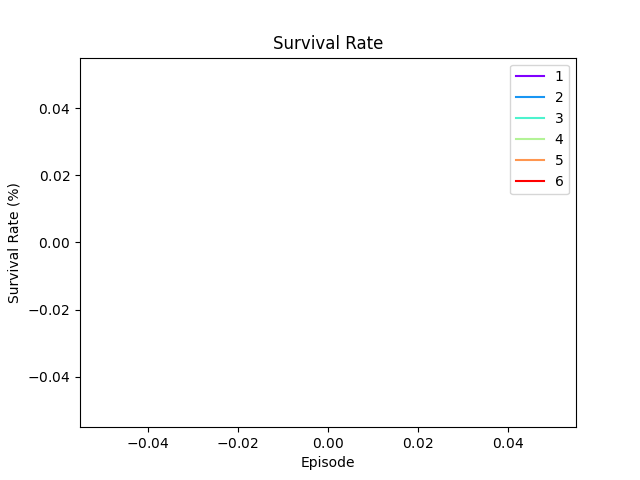
\includegraphics[width=.45\textwidth]{graphs/layers/survival_rate.png}} 
	\vfill
	\subfloat{}{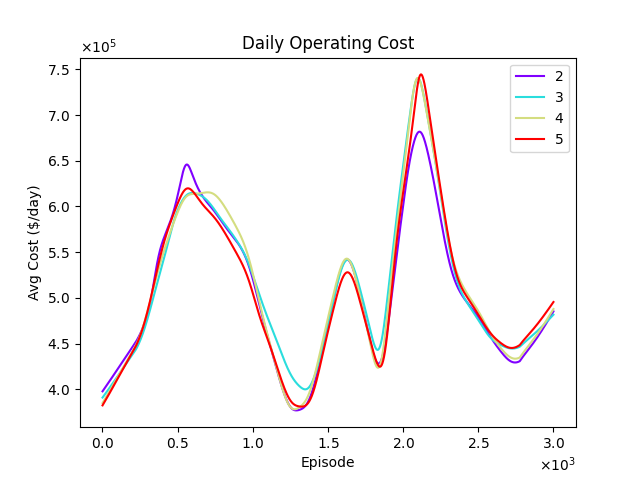
\includegraphics[width=.45\textwidth]{graphs/layers/daily_cost.png}} \hskip1ex
	\subfloat{}{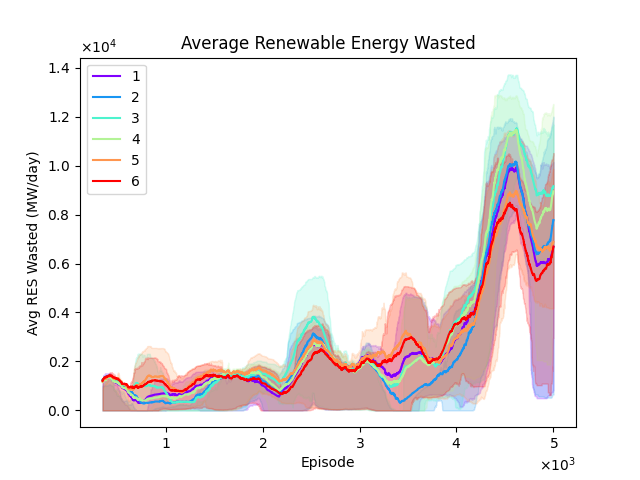
\includegraphics[width=.45\textwidth]{graphs/layers/res_wasted.png}} 
	\caption{Training Results of models with 1, 2 and 3 \ac{GAT} Heads}
	\label{fig:gat-heads-train}
\end{figure}

\begin{comment}
\begin{table}[ht]
	\centering
	\begin{tabularx}{\textwidth}{|l|X|X|X|X|X|}
		\hline
		\textbf{Model} & \textbf{Avg. Accumulative Reward}& \textbf{Avg. Length (Steps)} & \textbf{Avg Daily Operating Cost (€)} & \textbf{Avg. Renewables Wasted (MW/day)} & \textbf{Total Time (Seconds)}\\
		\hline
		1 & & & & & \\
		2 & & & & & \\
		3 & & & & & \\
		\hline
	\end{tabularx}
	\caption{Validation Results of the Experiments concerning Limit Infeasible Curtail Actions.}
	\label{fig:curtail-val}
\end{table}
\end{comment}